\documentclass{beamer}
\usepackage{risk231}   % shared preamble: packages, theorems, colours, timelines

\setchapter{1}         % sections numbered 1.1, 1.2, ...

\title{RISK 231: Introduction}

\begin{document}
\maketitle

%======================================================================
\section{Course introduction}
%======================================================================

\begin{frame}{My Introduction}
\begin{itemize}
  \item Professional Intro
  \begin{itemize}
    \item \href{https://www.linkedin.com/in/himchan-jeong-b5b65110a/?originalSubdomain=ca}{LinkedIn Profile}
    \item \href{https://scholar.google.com/citations?user=WOqS7-8AAAAJ&hl=en}{Publication List}
    \item Business Administration/Mathematics Major at Seoul National University
    \item Assistant Manager in DB Insurance (South Korea)
  \end{itemize}
  \vspace{0.6em}
  \item Personal Intro
  \begin{itemize}
    \item (Used to) play the guitar
    \item Love to eat, cook to eat, work out to eat
  \end{itemize}
\end{itemize}
\end{frame}

\begin{frame}{Required Materials}
\begin{itemize}
  \item Note that you can download Office 365 for free as an SFU student.
  \vspace{0.6em}
  \item R and RStudio are also free.
  \vspace{0.6em}
  \item If possible, I would encourage you to bring your own laptop so that
        you can practise along with the lectures during class time.
\end{itemize}
\end{frame}

%======================================================================
\section{Why do actuaries need to know tools for data-driven decision making?}
%======================================================================

\sectionframe

% Candy bars as a faded background behind the text
{
\usebackgroundtemplate{%
  \tikz\node[opacity=0.35,inner sep=0]{\includegraphics[width=\paperwidth,height=\paperheight]{ch01/candy_bars}};}
\begin{frame}{What does an actuary do?}
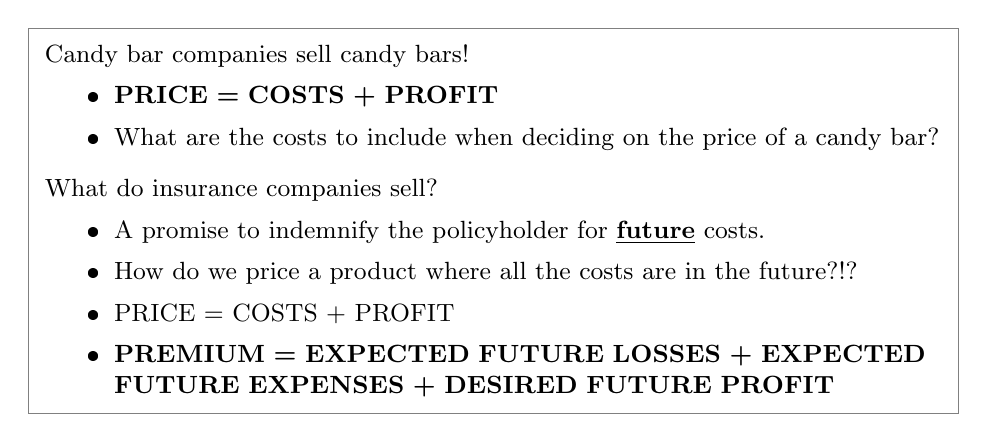
\begin{tikzpicture}
\node[fill=white, fill opacity=0.92, text opacity=1, draw=gray,
      text width=0.94\textwidth, inner sep=6pt, font=\small] {%
  Candy bar companies sell candy bars!
  \begin{itemize}
    \item \red{\textbf{PRICE = COSTS + PROFIT}}
    \item What are the costs to include when deciding on the price of a candy bar?
  \end{itemize}
  \vspace{0.4em}
  What do insurance companies sell?
  \begin{itemize}
    \item A promise to indemnify the policyholder for \underline{\textbf{future}} costs.
    \item How do we price a product where all the costs are in the future?!?
    \item PRICE = COSTS + PROFIT
    \item \red{\textbf{PREMIUM = EXPECTED FUTURE LOSSES + EXPECTED FUTURE EXPENSES
          + DESIRED FUTURE PROFIT}}
  \end{itemize}
};
\end{tikzpicture}
\end{frame}
}

\begin{frame}{What does an actuary do?}
\centering
\begin{tikzpicture}
  \node[inner sep=0] (img) {\includegraphics[width=0.82\textwidth]{ch01/fortune_teller}};
  % text inside the crystal ball
  \node[font=\large\bfseries, text=blue!60!black, align=center]
       at ($(img.south)!0.21!(img.north)+(0.1,0)$) {EXPECTED\\FUTURE\\COSTS};
  % speech bubble
  \node[rectangle callout, draw=blue!60!black, thick, fill=white, rounded corners=4pt,
        align=center, font=\small, text=blue!60!black, inner sep=6pt,
        callout absolute pointer={($(img.north)!0.45!(img.center)+(0.5,0)$)}]
       at ($(img.north east)+(-0.4,-0.1)$) {Your Premium\\is\ldots};
\end{tikzpicture}
\end{frame}

\begin{frame}{Why do actuaries need to know programming?}
\centering
\begin{tikzpicture}[
    box/.style={draw=black!70, thick, align=center},
    use/.style={ellipse, draw=black!60, fill=white, minimum width=2.6cm,
                minimum height=0.8cm, inner sep=0pt, align=center, font=\tiny},
    input/.style={box, text width=1.9cm, minimum height=1.2cm, font=\scriptsize},
    up/.style={-{Latex}, thick, black!70}]
  % main flow
  \node[box, minimum width=1.6cm, minimum height=1.6cm, font=\small] (hist) at (0,0.3) {Historical\\Data};
  \node[single arrow, draw=black!70, thick, single arrow head extend=0.2cm,
        minimum height=3.3cm, text width=2.1cm, align=center, font=\scriptsize,
        anchor=west] (adj) at (0.9,0.3) {Adjust data to the future time period};
  \node[box, text width=1.8cm, minimum height=3.0cm, font=\small, anchor=west]
       (pred) at (4.3,0.3) {Use adjusted data to predict future costs};
  % applications
  \foreach \t [count=\i] in {Ratemaking, Reserving, Planning, Book\\Management,
                             Underwriting, Investment\\Strategy, Claims\\Analytics, And more\ldots}
    \node[use] at ({7.75+0.35*mod(\i,2)}, {2.95-0.72*(\i-1)}) {\t};
  % inputs to the adjustment
  \node[input] (b1) at (0.75,-2.35) {Industry Benchmarks \& Trends};
  \node[input] (b2) at (2.85,-2.35) {Informed Assumptions};
  \node[input] (b3) at (4.95,-2.35) {Trends \& patterns from historical data};
  \coordinate (abot) at ($(adj.west)+(0,-0.62)$);   % bottom edge of the arrow body
  \draw[up] (b1.north) -- ($(abot)+(0.5,0)$);
  \draw[up] (b2.north) -- (b2.north |- abot);
  \draw[up] (b3.north) -- ($(abot)+(3.2,0)$);
\end{tikzpicture}
\end{frame}

\begin{frame}{Why do actuaries need to know tools for data-driven decision making?}
\centering
\begin{tikzpicture}[
    tool/.style={single arrow, draw=black!70, thick, single arrow head extend=0.15cm,
                 minimum height=4.9cm, text width=4.3cm, align=center, font=\tiny,
                 anchor=west},
    feed/.style={-{Latex}, very thick}]
  \node[draw=black!70, thick, minimum width=1.5cm, minimum height=2.6cm,
        align=center, font=\small] (hist) at (0,0.6) {Historical\\Data};
  % three routes from data to tools
  \node[tool] (a1) at (0.9, 1.9) {Smaller dataset, ad hoc analysis};
  \node[tool] (a2) at (0.9, 0.6) {Medium dataset, repeated processes};
  \node[tool] (a3) at (0.9,-0.8) {Large datasets, repeated processes, ad hoc analysis,
                                  predictive modeling, exploratory data analysis};
  \node[anchor=west, inner sep=0] (excel)  at (5.9, 1.9) {\includegraphics[height=0.85cm]{ch01/logo_excel}};
  \node[anchor=west, inner sep=0] (access) at (5.9, 0.6) {\includegraphics[height=0.85cm]{ch01/logo_access}};
  \node[anchor=west, inner sep=0] (rlogo)  at (5.9,-0.8) {\includegraphics[height=0.95cm]{ch01/logo_r}};
  \node[anchor=west, inner sep=0] (py)     at (rlogo.east) {\includegraphics[height=0.95cm]{ch01/logo_python}};
  \node[anchor=west, inner sep=0] (sas)    at (py.east)    {\includegraphics[height=0.95cm]{ch01/logo_sas}};
  % SQL: data preparation feeding every tool
  \node[inner sep=0] (sql) at (2.4,-2.45) {\includegraphics[height=0.6cm]{ch01/logo_sql}};
  \node[below=1pt of sql, font=\scriptsize, align=center] {Data prep, querying, filtering, etc.};
  \draw[-{Latex}, thick, black!70, rounded corners=6pt]
       (hist.south) |- (sql.west);
  % coloured feeds routed around the right so they do not cross the text
  \draw[feed, dgreen, rounded corners=4pt]
       ($(sql.east)+(0,0.1)$) -| (9.15,1.9) -- (excel.east);
  \draw[feed, red!75!black, rounded corners=4pt]
       (sql.east) -| (8.9,0.6) -- (access.east);
  \draw[feed, blue!60!black, rounded corners=4pt]
       ($(sql.east)+(0,-0.1)$) -| (py.south);
\end{tikzpicture}
\end{frame}

%======================================================================
\section{Remarks}
%======================================================================

\begin{frame}{Some remarks}
\begin{itemize}
  \item While the course has been designed primarily to equip actuarial students
        with the computational skills they need, these skills are in fact versatile
        and can be used in any profession with office work.
  \vspace{0.5em}
  \item Note that MS Access is not available with SFU's Office 365 license, so it
        is not covered in this class -- in my understanding, MS Access is a version
        of a SQL application with better visualization.
  \vspace{0.5em}
  \item I think the most important reason that you need to learn Excel is\ldots
\end{itemize}
\vspace{1em}
{\Large \orange{\textbf{To avoid unnecessary overtime work and sneak out from your
workplace on time!}}\par}
\end{frame}

\begin{frame}{Suggestion for actuarial students}
\begin{itemize}
  \item I would strongly suggest that you
  \begin{itemize}
    \item pass SOA Exam P (STAT 270 + $\alpha$) -- costs USD 260,
    \item pass SOA Exam FM (ACMA 201) -- costs USD 260,
    \item and find a co-op position as an actuarial student.
  \end{itemize}
  \vspace{0.5em}
  \item After you have finished your first co-op, you can decide whether you would
        like to stay in the profession or look for another career. (Anyway, having
        one co-op opportunity does not hurt at all!)
  \vspace{0.5em}
  \item It is known that without one or two actuarial exams, it is not easy to
        secure an actuarial co-op (two is preferable).
\end{itemize}
\end{frame}

\end{document}
